\documentclass[twocolumn]{article}
\usepackage[utf8]{inputenc}
\usepackage[english]{babel}
% \usepackage[left=2.5cm,right=2.5cm,top=3cm,bottom=3cm]{geometry}
\usepackage[T1]{fontenc}
\usepackage[os=mac, mackeys=symbols]{menukeys}
\usepackage{graphicx}
\graphicspath{{plots/}{../img/}{tegninger/}}
\usepackage{xspace}
\usepackage[noadjust]{cite}
\usepackage{caption}
\usepackage{subcaption}
\usepackage{booktabs}
\usepackage{cancel}
\usepackage{subcaption}
\usepackage{float}
\usepackage{amsmath}
\usepackage{enumerate} % bedre enumeration
\usepackage{enumitem}
\usepackage{amssymb}
\usepackage{amsthm}
\usepackage{makecell}
\usepackage{algorithm}
\usepackage{algpseudocode}
\usepackage{listings}
\usepackage{minted}
\usepackage[all]{xy}
\usepackage{hyperref}
\usepackage[nameinlink,noabbrev]{cleveref}
\usepackage{fancyhdr}
\usepackage{lastpage}

\pagestyle{fancy}
\fancyhf{}
\rfoot{\centering Page \thepage \hspace{1pt} of \pageref{LastPage}}

\lstset{
    language=C++,
    basicstyle=\ttfamily,
    keywordstyle=\color{blue}\ttfamily,
    stringstyle=\color{red}\ttfamily,
    commentstyle=\color{gray}\ttfamily,
    morecomment=[l][\color{magenta}]{\#},
    showstringspaces=false,
    numbers=left,
    tabsize=2,
    breaklines=true,
    breakatwhitespace=false,
}

\lstset
{ %Formatting for code in appendix
    % basicstyle=\footnotesize,
    numbers=left,
    stepnumber=1,
    showstringspaces=false,
    tabsize=2,
    breaklines=true,
    breakatwhitespace=false,
}
\usepackage{cite}
\usepackage{mathtools}
\usepackage{pdfpages}
% \usepackage[framemethod=TikZ]{mdframed}
% \mdfdefinestyle{TLO}{
%     innertopmargin=\baselineskip,
%     innerbottommargin=\baselineskip,
%     innerrightmargin=20pt,
%     innerleftmargin=20pt,}
% \usepackage[parfill]{parskip}  % ingen indent ved ny paragraf

\DeclarePairedDelimiter\ceil{\lceil}{\rceil}
\DeclarePairedDelimiter\floor{\lfloor}{\rfloor}
\DeclareMathOperator{\EX}{\mathbb{E}}
\DeclareMathOperator{\prob}{P}
\DeclareMathOperator{\RR}{\mathbb{R}}
\DeclareMathOperator{\NN}{\mathbb{N}}
\DeclareMathOperator{\CC}	{\mathbb{C}}
\DeclareMathOperator{\ZZ}{\mathbb{Z}}
\newcommand{\abs}[1]{\left|#1\right|}
\newcommand{\brac}[1]{\left\{#1\right\}}
\newcommand{\sqrbrac}[1]{\left[#1\right]}
\newcommand{\paren}[1]{\left(#1\right)}
\newcommand{\normlines}[1]{\left\Vert#1\right\Vert}
\newcommand{\mtx}[1]{\textbf{#1}}

\newcommand{\note}[1]{\textcolor{red}{#1}\\}

%%% FORMATTING %%%
\usepackage{enumitem}
\usepackage{titlesec}
\titlespacing*{\section}{0pt}{0.8\baselineskip}{0.3\baselineskip}
\titlespacing*{\subsection}{0pt}{0.6\baselineskip}{0.3\baselineskip}
\titleformat{\section}
  {\normalfont\Large\bfseries}{\thesection}{1em}{}
\titleformat{\subsection}
  {\normalfont\large\bfseries}{\thesubsection}{1em}{}

\usepackage{titling}
\setlength{\droptitle}{-6em} 
\setlength{\columnsep}{0.55in}

% \usepackage{fancyhdr}
% \usepackage{lastpage}
% \usepackage{multicol}
\usepackage{blindtext}

\usepackage[a4paper,
            bindingoffset=0.2in,
            left=0.85in,
            right=0.85in,
            top=1.5in,
            bottom=1.5in,
            footskip=.25in]{geometry}

%%% TITLE%%%
\title{A Single Pass Scan Using Lookback}
\author{dwp992 \& lsh789}
\date{November 2023\vspace{2ex}}

\begin{document}

\maketitle
\thispagestyle{fancy}

\section{Introduction}

\section{Background}
\label{sec:background}

This project is based on the paper "Single-pass Parallel Prefix Scan with Decoupled Look-back" paper. %\cite{SPS_paper}
In this paper the authors go through explaining their implementation of a single pass scan, meaning we can scan with only 2 global IO accesses per element. (Not counting a few extra needed per block). The important part of the algorithm they introduce, is the decoupled lookback scan, that will scan over what previous blocks have gotten. The paper also proposes a number of optimisations, some of then we implemented and some of them will be discussed later on.

\subsection{Decoupled lookback}

Normally when we would do a scan we would need 3 global IO accesses per element, since we would first need a read, when calculating the reduction of each block and scanning over the result of these, this result will then be used in a second pass through were we then scan each block while adding the prefix we found from the reduction/block-level-scan this gives us another global read. And finally we need to write the result. What we can see from this normal implementation is that we 2 of the 3 global accesses are reading the same memory, the only problem is that we are reading it with bad temporal locality, so we can not keep the data. This is what we try to fix by doing a single-pass scan, since we only pass through the data once, we only do one global read. And then we calculate the reduction and result right away.

One of the issues with this way of implementing it. Is that we now have a dependency between the blocks, so in order for block 2 to calculate the result of it's scan, it needs the prefix value from block 1. In the paper they then introduce the lookback algorithm that lets the blocks update a global array with their prefix and aggregate values that future blocks then can use. This is done by the aggregate value being just a reduction of all the values in the block, and the prefix can be found by adding this aggregate to the previous blocks prefix. But for this we also need to ensure that the blocks are being calculated in certain order, so we do not just have all calculating threads waiting for block 1, that is in queue to being spawned, the paper suggest a dynamic scheduling of the blocks, which we utilised in our implementation.

\note{Bør man gå mere i dybden med aggrgate flag og prefix array, og lave en helt down to earth definition af dem : Jeg synes bare vi skal gøre det kort.}

\note{Maybe add the some text about the properties discussed in the paper, and what effect they have.}

\section{Our implementation}
\note{Bør vi tilføje lidt om hvordan vi håndterer dynamisk ID? : Yes, det har jeg gjort nu}
\label{Sec:Implementation}
This section describes the lookback algorithm we've implemented, the kernel that executes the scan, and the associated functions we've defined. Listing \ref{lst:lookbackKernel} describes the lookback kernel. Listing \ref{lst:lookbackScan} contains the code for our lookback algorithm.

\subsection{The Lookback Scan Kernel}
\label{sec:impl-lookback-kernel}
Listing \ref{lst:lookbackKernel} takes pointers to the input and output arrays, along with a size. We also pass as arguments 4 pointers to different global memory locations. The first is a dynamic ID that is shared across blocks. The second, third, and fourth are pointers to the flag array, aggregate array, and inclusive prefix array described in section \ref{sec:background}. The arrays are implemented using the \verb|volatile| keyword to ensure that memory is visible for all threads as soon as it's written, and the dynamic ids are handled using atomic additions. Specifically, the \verb|atomicAdd| function is used to add to the global variable and return the value before adding. Line 9-10 initializes the shared memory that we'll need. We create a shared array of size $Q * B$ and a shared buffer of size $B$. The shared array accompanying each block is reserved for part of the array the block scans. The shared buffer stores scans performed by each thread on \verb|Q| elements. The kernel code contains 6 different device functions:
\begin{enumerate}[leftmargin=*]
    \itemsep0em
    \item \verb|copyGlb2Shr| - Copies memory from global to shared memory in a coalesced fashion. Equivalent to the function used in assignment 2.
    \item \verb|threadScan| - Each thread scans $Q$ elements from the shared memory and writes the resulting value to the shared buffer at the index equal to the thread id.
    \item \verb|blockScan| - Performs an inclusive scan equivalent to the optimized warp scan from assignment 2.
    \item \verb|threadAdd| - Adds the correct inclusive prefix to all values in the shared memory. After this function call, all values in shared memory have values representing an inclusive scan for the block only.
    \item \verb|lookbackScan| - The lookback scan function looks through the flag, aggregate and prefix arrays to compute the appropriate exclusive prefix to add to the respective blocks shared memory. This function is described in detail in subsection \ref{sec:impl-lookback-alg}.
    \item \verb|threadAddVal| - Each thread adds the appropriate exclusive prefix to the $Q$ elements it's responsible for.
    \item \verb|copyShr2Glb| - Copies the shared memory to a location in the global array in a coalesced fashion. This is functionally equivalent to the one we used in assignment 2.
\end{enumerate}

Originally the design choice to use a separate shared memory buffer was made as it made the algorithm easier to construct in pseudo code. Furthermore, this choice makes the whole algorithm more easy to understand and explain. A potential drawback could be inefficiency in using $B*4$ extra bytes of shared memory per block, since if $B=1024$, this shared buffer would use $4*1024/49152 = 0.083\approx 8\%$ of the shared memory per block.

\subsection{The Lookback Algorithm}
\label{sec:impl-lookback-alg}

In accordance with section \ref{sec:background} we have implemented the lookback algorithm using 3 different arrays in global memory: A flag array, an aggregate array, and an inclusive prefix array. this section covers the lookback version where only 1 thread computes the exclusive prefix and updates its own aggregate value and inclusive prefix values. The implementation of this can be seen in listing \ref{lst:lookbackScan}. The lines 11 to 34 are computed only for the final thread in the block.

Line 11-16 covers the case in which the dynamic id is 0 - We set both the aggregate value and the prefix value equal to the final value in the shared memory for the block. It then memory fences and then sets its flag to be P.

Line 18-34 covers the cases where the dynamic ids are greater than 0. First the aggregate value is set to the final value in the shared memory for the block. After a memory fence we set the flag value to A. We then define a \verb|grab_id| - an index of where we want values to add to our current aggregate value to produce an inclusive prefix. In line 25-29, while the flag at \verb|grab_id| is not P and the \verb|grab_id| is greater than zero, the aggregate value at \verb|grab_id| is added to an accumulating variable and the id is decremented. Finally, once a P flag is reached, the prefix value at the dynamic id is set to the current accumulation plus the prefix value at the \verb|grab_id|. After a fence, set the dynamic id flag to P.

Finally after a inter-block thread synchronization, in line 37, computed by all threads in the block, a prefix variable is created - this is the exclusive prefix value returned. It is computed by the prefix value minus the aggregate value accompanying the dynamic id.

\subsection{Parallelization of the lookback algorithm}


\subsection{SPS using an auxiliary block}

We also implemented the method mentioned in the old slides written by professor Henriksen, wherein the construction of the inclusive prefix array is done by one auxiliary block that is given the dynamic id of -1. As values in the aggregate array become available, this auxiliary block sequentially computes the prefix array. Blocks that have computed an aggregate value wait for the prefix value to be computed, and once it has the block adds the exclusive prefix to its section of the scanned array. If interested the code can be found in listing \ref{lst:aux_block}.


\section{Experiments}
\label{sec:experiments}
\subsection{Throughput for different array sizes}
Our first experiment was comparing our implementations

\begin{figure}
    \centering
    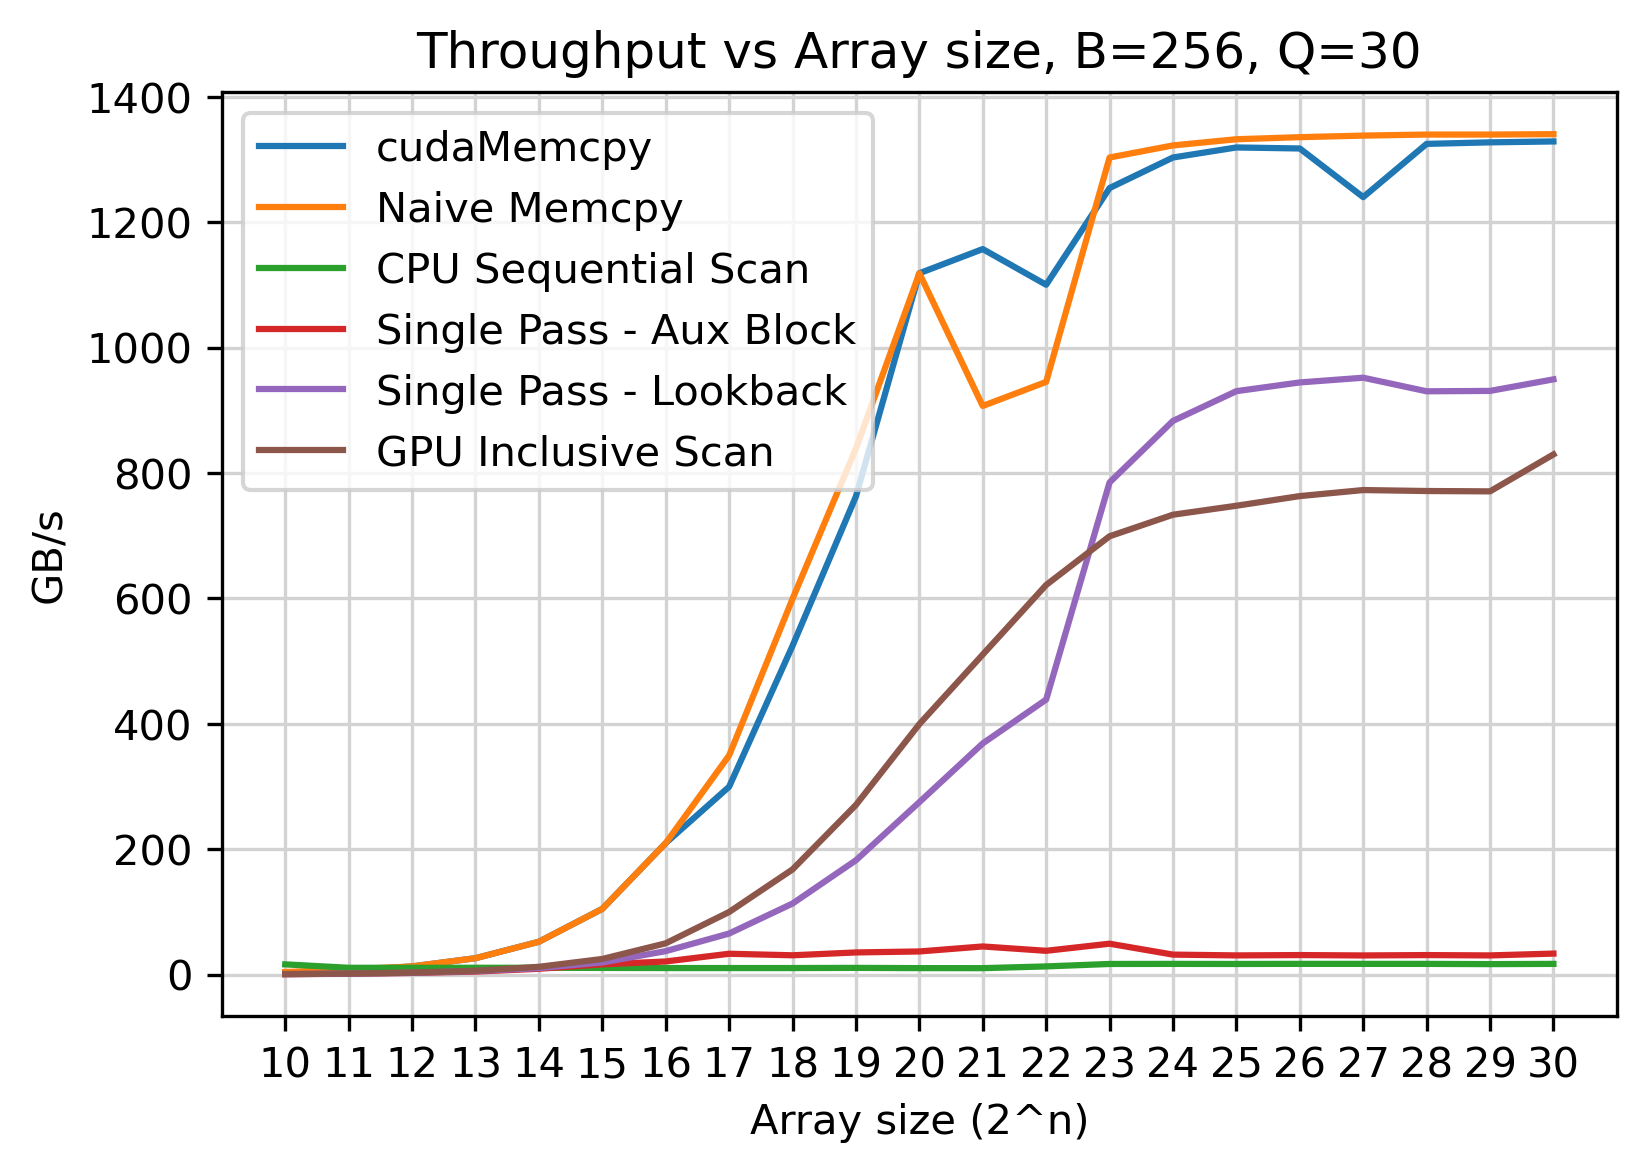
\includegraphics[width=\linewidth]{report/plots/throughput_vs_array_size_B256_Q30.png}
    \caption{Caption}
    \label{fig:enter-label}
\end{figure}

\begin{figure}
    \centering
    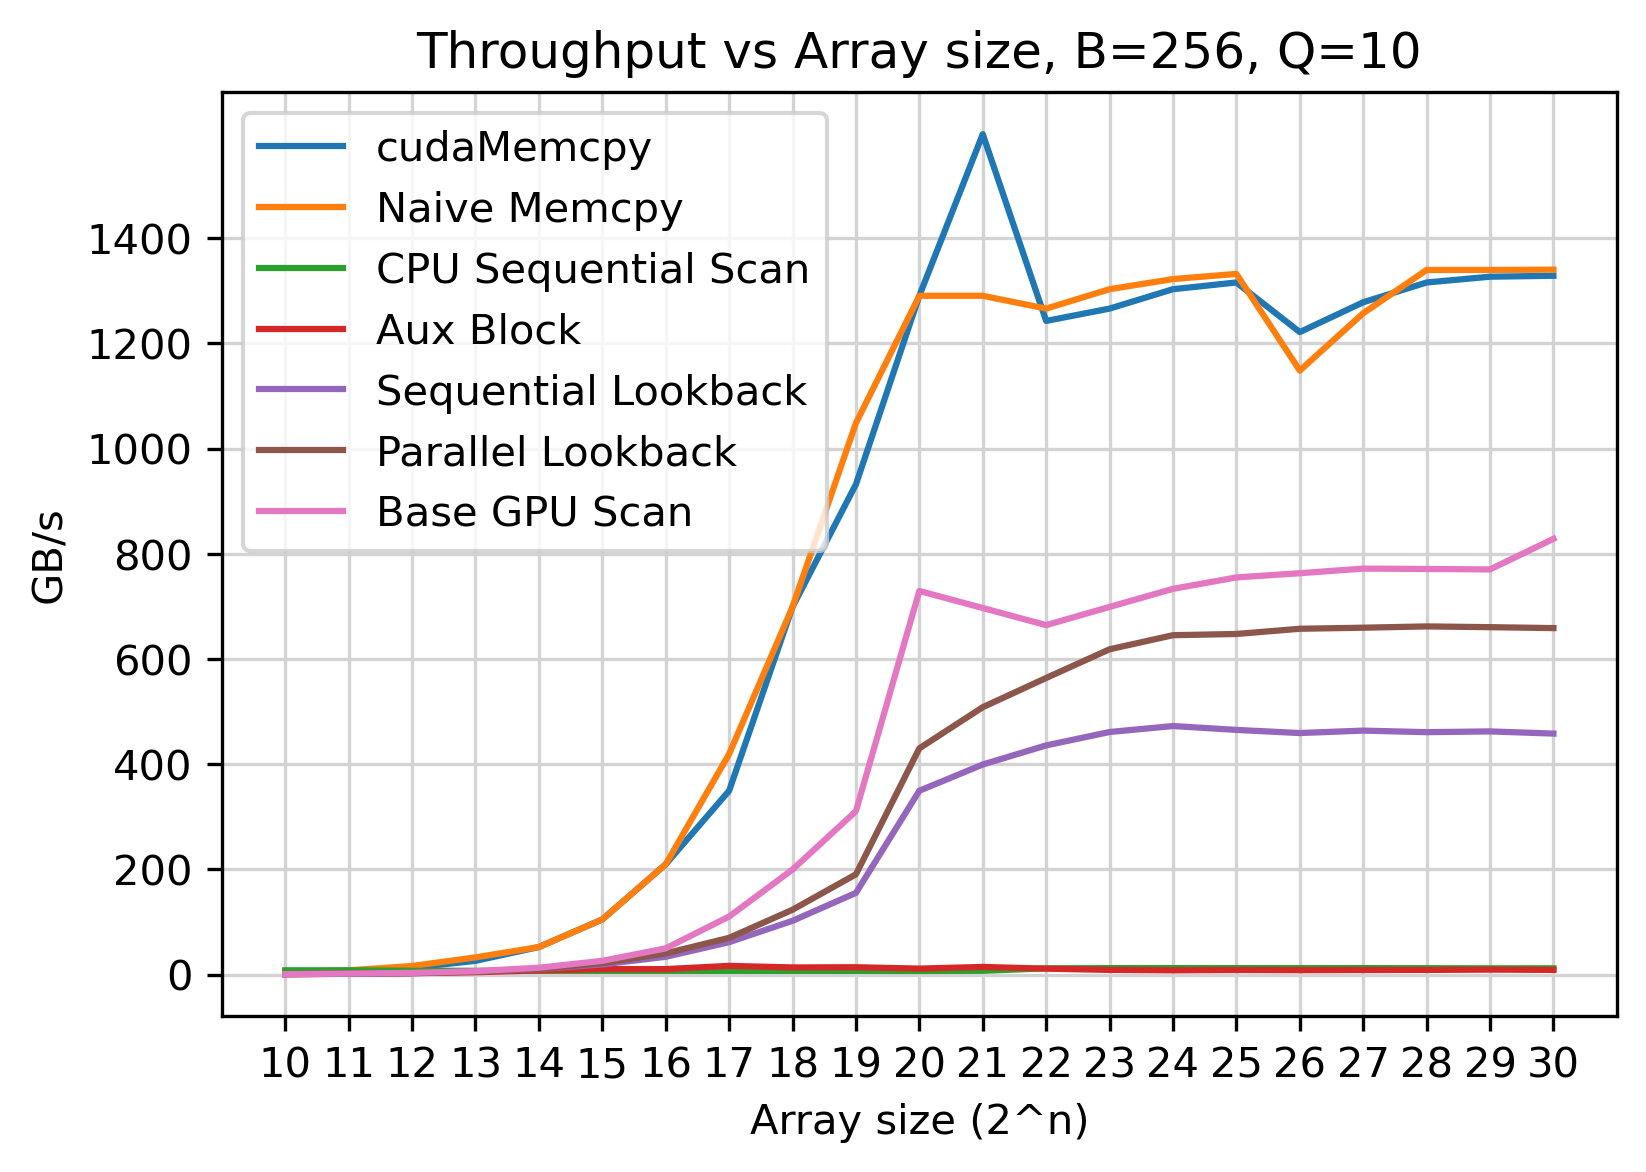
\includegraphics[width=\linewidth]{report/plots/throughput_vs_array_size_B256_Q10.png}
    \caption{Caption}
    \label{fig:enter-label}
\end{figure}

\begin{figure}
    \centering
    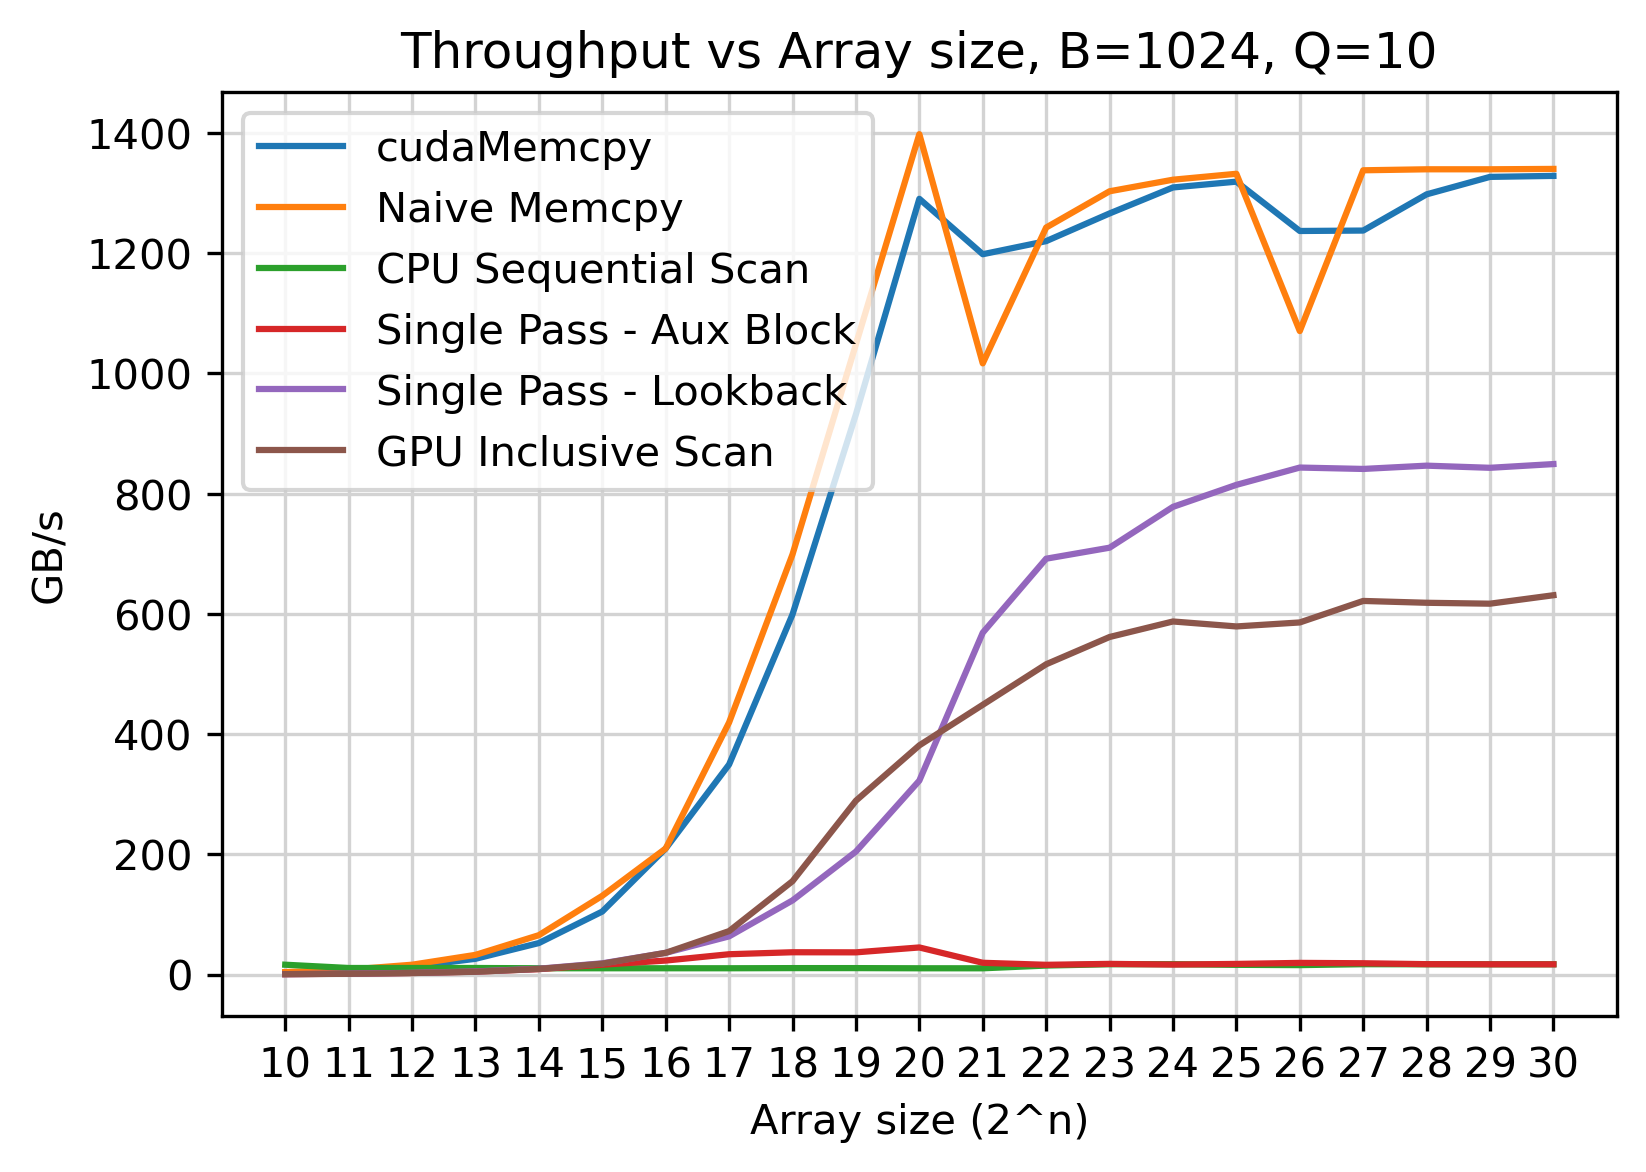
\includegraphics[width=\linewidth]{report/plots/throughput_vs_array_size_B1024_Q10.png}
    \caption{Caption}
    \label{fig:enter-label}
\end{figure}

\section{Future work or future improvements}
\note{Not sure what this section should be named.\\}
\note{Remember to reference the idea we mentioned earlier about not using a shared buffer for blockScan.}

\begin{figure*}
    \centering
    \begin{subfigure}{0.47\linewidth}
        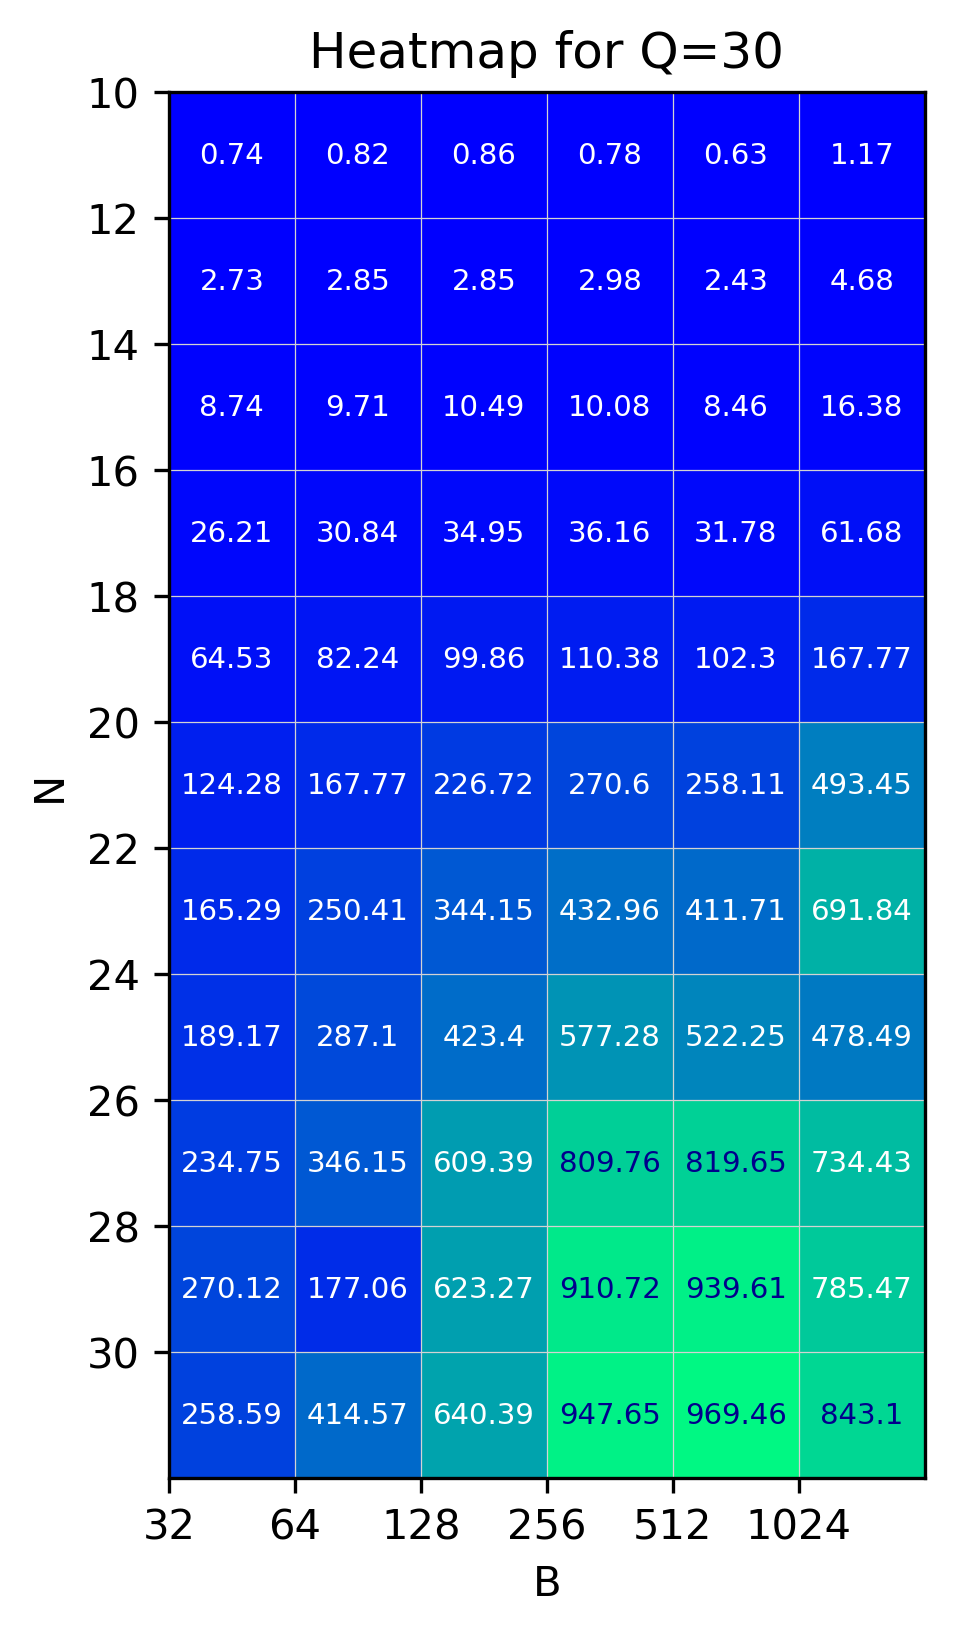
\includegraphics[width=\linewidth]{report/plots/heatmap_BvN_Q=30.png}
    \end{subfigure}
\end{figure*}

\onecolumn

\newpage

\section{Appendix}

\appendix

\section{Code for the lookback kernel}

% \newpage
\begin{lstlisting}[caption=Lookback kernel,label=lst:lookbackKernel]
template <typename T>
__global__ void SinglePassScanKernel2(T* d_in, T* d_out,
                                      const size_t N,
                                      int32_t* IDAddr,
                                      volatile uint32_t* flagArr,
                                      volatile T* aggrArr,
                                      volatile T* prefixArr) {
    // Allocate shared memory
    __shared__ T blockShrMem[Q * B];
    volatile __shared__ T blockShrBuf[B];

    // Step 1 get ids and initialize global arrays
    uint32_t tid = threadIdx.x;
    int32_t dynID = getDynID(IDAddr, tid);
    uint32_t globaloffset = dynID * B * Q;

    // Step 2 copy the memory the block will scan into shared memory.
    copyGlb2Shr<T>(globaloffset, N, T(), d_in, blockShrMem, tid);

    // Step 3 Do the scan on the block
    // First scan each thread
    threadScan<T>(blockShrMem, blockShrBuf, tid);

    // Do the scan on the block level
    blockScan<T>(blockShrBuf, tid);

    // Save the result in shrmem.
    threadAdd<T>(blockShrMem, blockShrBuf, tid);

    // Step 4 use lookback scan to find the inclusive prefix value
    T prefix =
        lookbackScan<T>(aggrArr, prefixArr, flagArr, blockShrMem, dynID, tid);

    // Step 5 Sum the prefix into the scan
    threadAddVal<T>(blockShrMem, prefix, tid, dynID);

    // Step 6 Copy the result into global memory
    copyShr2Glb<T>(globaloffset, N, d_out, blockShrMem, tid);
}
\end{lstlisting}

\newpage

\section{Code for the lookback scan function}
\begin{lstlisting}[caption=Lookback kernel,label=lst:lookbackScan]
template<typename T>
__device__ inline T lookbackScan(volatile T* agg_mem,
                                 volatile T* pref_mem,
                                 volatile uint32_t* flag_mem,
                                 T* shr_mem, uint32_t dyn_idx,
                                 uint32_t tid) {
    #define X 0
    #define A 1
    #define P 2
	// Handle lookback differently depending on dynamic id.
    if (tid == B - 1 && dyn_idx == 0) {
		T agg_val = shr_mem[(Q - 1) * B + tid];
		agg_mem[dyn_idx] = agg_val;
        pref_mem[dyn_idx] = agg_val;
        __threadfence();
        flag_mem[dyn_idx] = P;

    } else if (tid == B - 1 && dyn_idx > 0) {
		T agg_val = shr_mem[(Q - 1) * B + tid];
        agg_mem[dyn_idx] = agg_val;
        __threadfence();
        flag_mem[dyn_idx] = A;
        uint32_t grab_id = dyn_idx - 1;
        // isnt there a bug here when we encounter an X?
        while (flag_mem[grab_id] != P) {
            if (flag_mem[grab_id] == A && grab_id > 0) {
                agg_val = agg_mem[grab_id] + agg_val;
                grab_id--;
            }
        }
		pref_mem[dyn_idx] = agg_val + pref_mem[grab_id];
        __threadfence();
        flag_mem[dyn_idx] = P;
    }

	__syncthreads();
	T prefix = pref_mem[dyn_idx] - agg_mem[dyn_idx];

    return prefix;
}
\end{lstlisting}



\end{document}
